\documentclass[conference]{IEEEtran}

\usepackage[T1]{fontenc}
\usepackage[utf8]{inputenc}
\usepackage{amsmath,amssymb,bm}
\usepackage{booktabs,multirow,array,tabularx,ragged2e}
\usepackage{graphicx}
\usepackage{xcolor}
\usepackage{cite}
\usepackage{microtype}
\usepackage{siunitx}
\usepackage{enumitem}
\usepackage[hidelinks]{hyperref}

\newcolumntype{C}[1]{>{\centering\arraybackslash}p{#1}}
\newcolumntype{L}[1]{>{\RaggedRight\arraybackslash}p{#1}}
\renewcommand{\arraystretch}{1.18}
\setlength{\tabcolsep}{4pt}

\title{YogaLLaVA: Geometry-Conditioned Vision--Language Reasoning for Yoga Pose Understanding}

\author{
\IEEEauthorblockN{Manav Barot, Sadamori Kojaku}
\IEEEauthorblockA{
School of Systems Science and Industrial Engineering\\
State University of New York (SUNY), Binghamton, NY, USA
}
}

\begin{document}
\maketitle

\begin{abstract}
Fine-grained yoga-pose understanding requires models to relate visual
appearance to explicit body geometry and domain-specific language. Existing
yoga datasets primarily support pose recognition and provide neither 3D body
measurements nor language supervision grounded in those measurements. We
introduce \textbf{YogaAlign}, a benchmark derived from Yoga-82 that augments
yoga images with SAM 3D Body reconstructions, interpretable joint- and
trunk-level descriptors, bilateral-symmetry measures, and instruction-style
annotations. YogaAlign contains 10,090 records: 6,000 image-specific
geometry-grounded question--answer pairs and 4,090 pose-level domain-knowledge
pairs.

We further propose \textbf{YogaLLaVA V3}, a geometry-conditioned
vision--language model that represents structured measurements as metric-aware
tokens and couples autoregressive language generation with continuous
angle-slot regression. On 521 held-out angle slots, YogaLLaVA V3 obtains a
teacher-forced MAE of $13.98^\circ$, an RMSE of $21.82^\circ$, and 57.01\%
accuracy within $10^\circ$ of the reconstruction-derived references. Under
free-running generation, it emits the correct number of numeric slots for
86.1\% of 310 geometry-grounded test records and achieves an MAE of
$17.65^\circ$ on the 160-record common-success subset shared by all evaluated
models. Because nearly all evaluated targets are supplied through the
structured geometry input, these experiments assess question-conditioned
measurement selection and expression rather than independent biomechanical
angle recovery from RGB images.
\end{abstract}

\begin{IEEEkeywords}
vision--language models; yoga pose understanding; 3D human mesh recovery;
geometry grounding; instruction tuning; Yoga-82
\end{IEEEkeywords}

\section{Introduction}
\label{sec:intro}

Human pose analysis is commonly formulated as keypoint localization, skeleton
recovery, or action recognition~\cite{cao2019openpose,sun2019deep}. These tasks
provide strong perceptual representations, but they do not directly answer
questions about how a body is configured, which side is more flexed, or how a
measured geometric property should be expressed in natural language. Such
questions require a model to connect image evidence with explicit body
measurements and linguistic reasoning.

Yoga is a particularly demanding setting for this problem. Many asanas are
distinguished by subtle differences in joint flexion, limb elevation, trunk
orientation, and bilateral symmetry. Yoga-82~\cite{verma2020yoga82} provides a
large and visually diverse benchmark for fine-grained recognition across 82
pose categories, but its supervision is limited to hierarchical category
labels. It does not provide reconstructed 3D bodies, interpretable geometric
descriptors, or question--answer annotations that connect a specific image to
its measured configuration.

Recent progress in monocular human mesh recovery and visual instruction tuning
offers a path toward such supervision. SAM 3D Body recovers articulated body
structure under the Momentum Human Rig representation from a single
image~\cite{yang2026sam3dbody}, while models such as LLaVA learn to follow
language instructions conditioned on visual input~\cite{liu2023visual}. A
direct combination, however, leaves two unresolved issues. First, dense mesh
outputs must be converted into compact and interpretable measurements. Second,
continuous geometric values must be integrated into language generation without
reducing numeric prediction to unconstrained text-token generation.

We address these issues through \textbf{YogaAlign} and \textbf{YogaLLaVA V3}.
YogaAlign augments Yoga-82 with SAM 3D Body reconstructions and a structured
taxonomy of angular, symmetry, trunk, and support descriptors. It further
provides two complementary annotation streams: pose-level domain-knowledge QA
derived from evidence-filtered textual sources and image-specific
geometry-grounded QA generated from explicit measurement paths. YogaLLaVA V3
then incorporates the angular subset of these measurements through ordered
\texttt{<GEO>} tokens. A dedicated \texttt{<ANGLE>} mechanism separates the
decision to emit a numeric slot from continuous scalar regression and feeds the
predicted value back into the autoregressive context.

Our contributions are threefold:
\begin{itemize}[leftmargin=1.2em,itemsep=2pt,topsep=3pt]
    \item We introduce \textbf{YogaAlign}, a geometry-grounded extension of
    Yoga-82 containing structured 3D-derived descriptors and 10,090 auditable
    instruction-style QA records across 82 asanas.
    \item We develop a two-stream annotation pipeline that combines
    evidence-conditioned yoga-domain knowledge with image-specific geometric
    paths, exact angular targets, rule-based validation, and provenance
    metadata.
    \item We propose \textbf{YogaLLaVA V3}, which integrates metric-aware
    geometry tokens, continuous angle-slot regression, and scalar feedback into
    a vision--language decoder, and evaluate both teacher-forced numeric routing
    and free-running generation.
\end{itemize}

\section{Related Work}
\label{sec:related}

\noindent\textbf{Human pose estimation and body reconstruction.}
Convolutional and transformer-based pose estimators have progressively improved
2D keypoint localization. Stacked Hourglass networks repeatedly fuse
bottom-up and top-down features~\cite{newell2016stacked}; Simple Baselines use a
ResNet backbone with deconvolutional prediction heads~\cite{xiao2018simple};
OpenPose introduces Part Affinity Fields for bottom-up multi-person
association~\cite{cao2019openpose}; HRNet maintains high-resolution features
throughout the network~\cite{sun2019deep}; and ViTPose demonstrates the
effectiveness of transformer backbones for pose estimation~\cite{xu2022vitpose}.

Moving beyond 2D joints, SMPL provides a parametric representation of body pose
and shape~\cite{loper2015smpl}. HMR regresses SMPL parameters from a single
image~\cite{kanazawa2018end}, SPIN combines regression with optimization-based
model fitting~\cite{kolotouros2019spin}, CLIFF incorporates person location in
the full image~\cite{li2022cliff}, and HMR 2.0 uses transformer-based
representations for improved in-the-wild reconstruction~\cite{goel2023humans}.
SAM 3D Body extends this line with full-body recovery under the MHR
representation~\cite{yang2026sam3dbody}. We use reconstruction as an annotation
mechanism: dense outputs are converted into interpretable measurements that
ground downstream language supervision.

\noindent\textbf{Action quality and pose correction.}
Action quality assessment estimates how well an action is performed rather
than only recognizing its category~\cite{lei2019survey}. Prior work includes
cross-action quality scoring~\cite{parmar2019action} and learning-based
assessment of rehabilitation exercises~\cite{liao2020deep}. Pose Tutor targets
explainable correction in yoga and related exercise domains by identifying
joint-angle contributions to pose predictions~\cite{dittakavi2022posetutor}.
These approaches typically produce scores, error indicators, or localized
corrections. Our focus is complementary: we construct language supervision
whose numeric statements remain traceable to explicit image-specific
measurements.

\noindent\textbf{Vision--language learning and visual QA.}
CLIP learns transferable image--text representations through contrastive
pretraining~\cite{radford2021clip}. Flamingo supports few-shot multimodal
generation~\cite{alayrac2022flamingo}, while BLIP-2 connects frozen image
encoders and language models through a Q-Former~\cite{li2023blip2}. LLaVA and
InstructBLIP demonstrate the effectiveness of visual instruction
tuning~\cite{liu2023visual,dai2023instructblip}. Qwen2-VL further supports
dynamic-resolution visual processing~\cite{wang2024qwen2vl}. Standard VQA
benchmarks such as VQAv2 and GQA emphasize objects, attributes, and relational
reasoning~\cite{goyal2017vqav2,hudson2019gqa}; they do not provide supervision
for selecting and verbalizing continuous human-body measurements. YogaAlign is
designed to fill this gap.

\noindent\textbf{Human pose datasets.}
COCO and MPII provide large-scale 2D keypoint annotations
~\cite{lin2014coco,andriluka2014mpii}; Human3.6M provides controlled 3D human
pose data~\cite{ionescu2014human36m}; and 3DPW provides in-the-wild 3D pose
annotations captured with inertial sensors and a moving camera
~\cite{vonMarcard2018}. Yoga-82 instead targets fine-grained yoga-pose
classification~\cite{verma2020yoga82}. YogaAlign builds on its category and
image diversity while adding reconstruction-derived measurements and
language-grounded supervision.

\section{YogaAlign Dataset}
\label{sec:dataset}

We construct \textbf{YogaAlign}, a geometry-grounded vision--language
benchmark that extends Yoga-82 with reconstructed 3D body structure,
interpretable geometric measurements, and instruction-style question--answer
(QA) annotations. The benchmark is designed to support reasoning beyond pose
recognition, including joint-angle interpretation, bilateral comparison,
regional alignment analysis, and pose-specific instructional knowledge. Its
construction comprises three stages: (i) monocular 3D body reconstruction,
(ii) extraction of structured geometric descriptors, and (iii) generation of
two complementary QA streams grounded in either pose-level textual knowledge
or image-specific geometry.

\subsection{Source Images and 3D Body Reconstruction}
\label{subsec:source_reconstruction}

\noindent\textbf{Yoga-82 source dataset.}
YogaAlign is built on Yoga-82~\cite{verma2020yoga82}, which contains 28,478
images spanning 82 fine-grained yoga-pose categories. The images were collected
from online sources and exhibit substantial variation in viewpoint, background,
illumination, clothing, practitioner appearance, and execution style. Yoga-82
is therefore a challenging substrate for geometry-aware reasoning: many poses
differ through subtle changes in limb articulation, trunk orientation, balance,
or bilateral symmetry. However, the original dataset provides only RGB images
and category labels; it does not include 3D body structure, geometric
measurements, or language annotations.

\noindent\textbf{Monocular body reconstruction.}
We recover a 3D body representation from each Yoga-82 image using the pretrained
SAM 3D Body model~\cite{yang2026sam3dbody}. Given an image $I$, the model
predicts an articulated body and surface mesh under the Momentum Human Rig
(MHR) representation. We retain the predicted mesh vertices and anatomical
keypoints required by the subsequent measurement pipeline. Figure~\ref{fig:sam3d_examples}
shows representative reconstructions across diverse asanas.

\begin{figure*}[!t]
    \centering
    \includegraphics[width=0.98\textwidth]{_ALL_CLASSES_GRID.png}
    \caption{Representative SAM 3D Body reconstructions for images from
    Yoga-82. The examples illustrate the diversity of articulated body
    configurations from which YogaAlign's geometric annotations are derived.}
    \label{fig:sam3d_examples}
\end{figure*}

The recovered bodies are treated as reconstruction-derived geometric proxies,
not as motion-capture or manually verified biomechanical ground truth. Their
accuracy may be affected by self-occlusion, foreshortening, loose clothing,
unusual inversions, left--right ambiguity, and monocular depth uncertainty.

\subsection{Geometric Measurement Extraction}
\label{subsec:geometric_measurements}

Dense meshes are expressive but unnecessarily high-dimensional for
language-grounded pose analysis. We therefore distill each reconstruction into
a compact set of anatomically interpretable descriptors. Before measurement,
we remove global translation by centering the vertices and keypoints at the mesh
centroid and use a fixed 3D coordinate convention with a consistent vertical
axis. Table~\ref{tab:geometric_metrics} groups the resulting descriptors by the
pose property they characterize.

\begin{table*}[t]
\centering
\caption{Taxonomy of geometric descriptors extracted from reconstructed 3D bodies.}
\label{tab:geometric_metrics}
\small
\setlength{\tabcolsep}{4pt}
\renewcommand{\arraystretch}{1.16}
\begin{tabularx}{\textwidth}{L{0.17\textwidth} L{0.25\textwidth} L{0.27\textwidth} X}
\toprule
\textbf{Group} & \textbf{Descriptors} & \textbf{3D computation} & \textbf{Reasoning target} \\
\midrule
Limb flexion &
Left/right knee and elbow flexion &
Interior angles of hip--knee--ankle and shoulder--elbow--wrist triplets &
Degree of flexion and left--right comparison. \\
Limb opening/elevation &
Left/right hip opening and shoulder elevation &
Angles between limb segments and torso-level reference axes &
Hip opening and arm elevation. \\
Trunk geometry &
Trunk tilt, lateral bend, twist, and neck alignment &
Pelvis--shoulder, shoulder--hip, and neck--torso directions &
Uprightness, lateral inclination, axial rotation, and head--torso consistency. \\
Bilateral symmetry &
Knee, elbow, and hip symmetry; shoulder and hip height offsets &
Left--right angular differences and normalized vertical offsets &
Symmetric or asymmetric execution across corresponding body regions. \\
Balance/support &
Stance width and body-center offset &
Ankle separation and horizontal displacement of the mesh center from the pelvis midpoint &
Base of support and lateral body shift. \\
\bottomrule
\end{tabularx}
\end{table*}

\noindent\textbf{Joint-angle descriptors.}
For three anatomical keypoints $\mathbf{p}_a$, $\mathbf{p}_b$, and
$\mathbf{p}_c$, we compute the angle centered at $\mathbf{p}_b$ as
\begin{equation}
\theta(a,b,c)=
\cos^{-1}\!\left(
\frac{(\mathbf{p}_a-\mathbf{p}_b)^{\top}(\mathbf{p}_c-\mathbf{p}_b)}
{\lVert\mathbf{p}_a-\mathbf{p}_b\rVert_2
 \lVert\mathbf{p}_c-\mathbf{p}_b\rVert_2}
\right).
\label{eq:joint_angle}
\end{equation}
Knee flexion is measured from the hip--knee--ankle triplet, whereas
elbow flexion is measured from the shoulder--elbow--wrist triplet. Hip opening
and shoulder elevation are computed relative to torso-level reference axes.
\begin{figure*}[t]
    \centering
    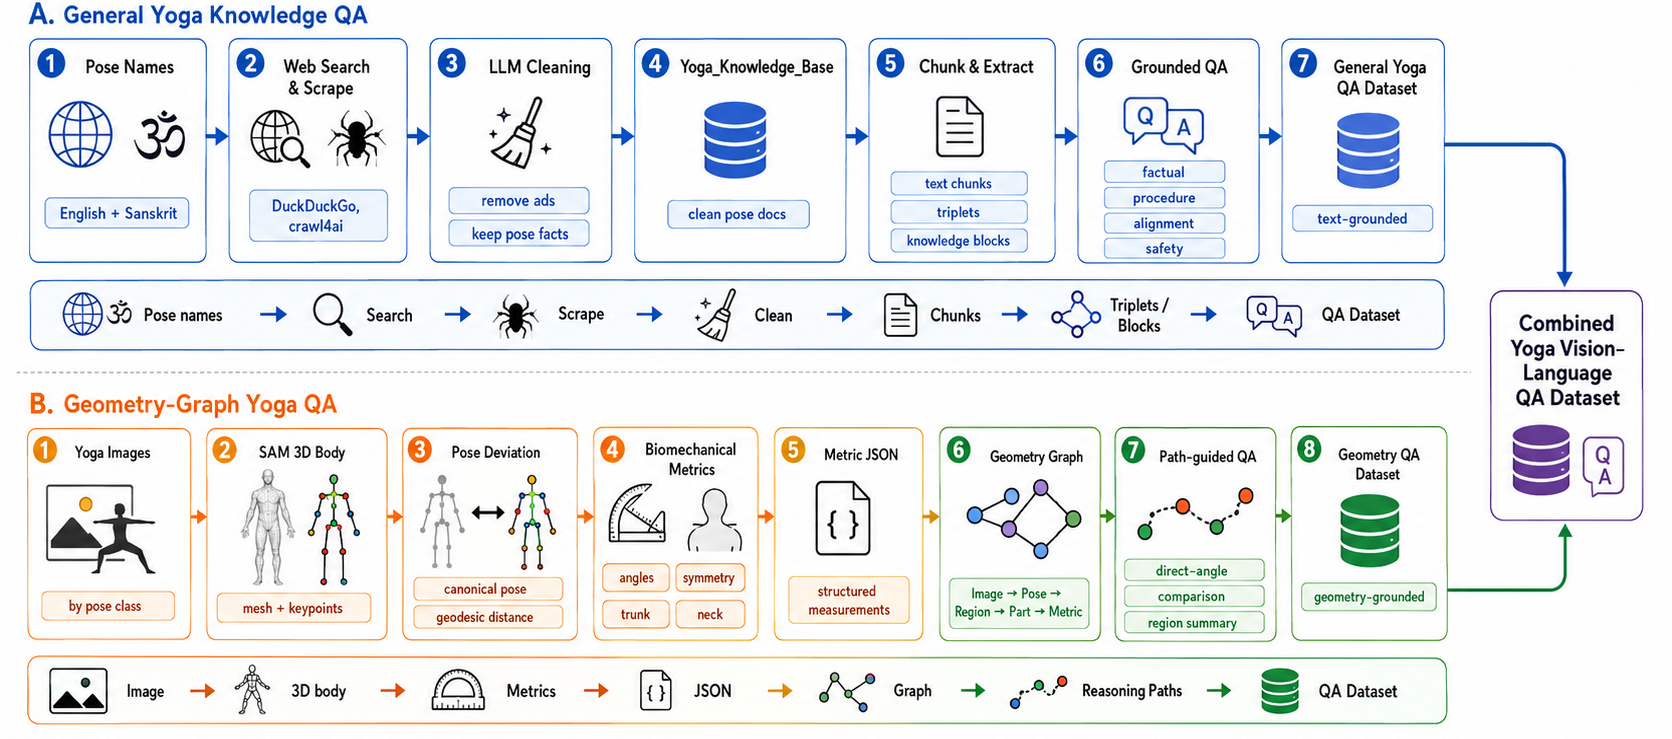
\includegraphics[width=\textwidth]{fig_dataset.png}
    \caption{\textbf{YogaAlign dataset-construction pipeline.}
    Pose-level domain knowledge and image-specific 3D geometry are processed
    through complementary pipelines to generate domain and geometry-grounded
    QA annotations.}
    \label{fig:dataset_pipeline}
\end{figure*}
\noindent\textbf{Trunk, symmetry, and support descriptors.}
Trunk measurements are derived from the pelvis--shoulder axis and the
shoulder--hip and neck--head directions. Bilateral descriptors quantify
differences between corresponding left and right measurements. Scale-dependent
quantities stance width, shoulder-height offset, and hip-height offset are
normalized by the vertical extent of the reconstructed mesh to reduce
sensitivity to body and reconstruction scale.

\noindent\textbf{Structured metric records.}
Each image is paired with a structured record containing the descriptor name,
anatomical region, numeric value, unit, definition, and discretized
interpretation state. Fixed thresholds map continuous measurements to
language-compatible states such as \emph{nearly straight}, \emph{deeply bent},
\emph{upright}, \emph{rotated}, or \emph{asymmetric}. These states facilitate
controlled verbalization while the underlying numeric values preserve exact
supervision. We use the measurements only as reconstruction-derived alignment
indicators for dataset construction; they are not intended as clinical,
diagnostic, or rehabilitation measurements.

\subsection{Question--Answer Annotation}
\label{subsec:qa_generation}

YogaAlign contains two complementary QA streams. The \emph{domain-knowledge}
stream captures pose-level semantic and instructional information that cannot
be inferred reliably from body geometry alone. The \emph{geometry-grounded}
stream verbalizes image-specific angular evidence extracted from the reconstructed
body. Table~\ref{tab:qa_annotation_overview} contrasts their evidence sources
and supervision targets.

\begin{table*}[t]
\centering
\caption{Complementary QA annotation streams in YogaAlign.}
\label{tab:qa_annotation_overview}
\small
\setlength{\tabcolsep}{4pt}
\renewcommand{\arraystretch}{1.15}
\begin{tabularx}{\textwidth}{L{0.19\textwidth} L{0.26\textwidth} L{0.30\textwidth} X}
\toprule
\textbf{QA stream} & \textbf{Primary evidence} & \textbf{Question scope} & \textbf{Supervision target} \\
\midrule
Domain knowledge &
Pose-specific text collected from online yoga sources &
Identity, benefits, contraindications, precautions, procedures, alignment cues,
modifications, breathing, mistakes, corrections, and sequencing &
Pose-level semantic and instructional reasoning. \\
Geometry grounded &
Degree-valued measurements extracted for an individual image &
Joint flexion, hip opening, shoulder elevation, trunk configuration, angular
symmetry, regional summaries, and measured-condition verification &
Image-specific measurement selection, comparison, interpretation, and numeric expression. \\
\bottomrule
\end{tabularx}
\end{table*}

\subsubsection{Domain-Knowledge QA Generation}
\label{subsubsec:domain_qa_generation}

\noindent\textbf{Pose-specific knowledge acquisition.}
For each of the 82 categories, we use Crawl4AI to retrieve and extract text from
pose-relevant online sources. The collected material is organized into one
document per asana. We retain information relevant to pose understanding and
instruction, including execution steps, alignment principles, modifications,
breathing cues, common mistakes, corrections, benefits, contraindications, and
precautions. Website boilerplate, navigation text, advertisements, author
biographies, publication metadata, product promotions, and generic marketing
language are excluded.

\noindent\textbf{Evidence structuring.}
Each pose document is divided into 5,000-character chunks with a 500-character
overlap. Rather than generating QA pairs directly from noisy source text, an
LLM-based extractor converts each chunk $c_i$ into two complementary evidence
representations:
\begin{equation}
(R_i,B_i)=E_{\phi}(c_i,p),
\label{eq:domain_extraction}
\end{equation}
where $p$ denotes the pose, $R_i$ is a set of compact relational facts, and
$B_i$ is a set of structured knowledge units. Relational facts encode atomic
subject--relation--object statements suited to concise factual questions.
Knowledge units retain multi-step or explanatory content suited to procedural,
alignment, safety, modification, breathing, sequencing, and correction
questions. Extraction is restricted to statements explicitly supported by the
current source chunk. In particular, unsupported claims that a pose cures or
treats a medical condition are not retained as factual supervision.

\begin{table*}[t]
\centering
\caption{Intermediate evidence representations for domain-knowledge QA generation.}
\label{tab:domain_knowledge_representation}
\small
\setlength{\tabcolsep}{4pt}
\renewcommand{\arraystretch}{1.15}
\begin{tabularx}{\textwidth}{L{0.21\textwidth} L{0.27\textwidth} L{0.28\textwidth} X}
\toprule
\textbf{Representation} & \textbf{Role} & \textbf{Typical content} & \textbf{Supported QA form} \\
\midrule
Relational facts &
Atomic, evidence-backed statements &
Names, difficulty, benefits, contraindications, precautions, props, muscles,
modifications, and related poses &
Concise factual and reverse-lookup questions. \\
Structured knowledge units &
Multi-sentence or multi-step evidence &
Procedures, alignment, safety, modifications, mistakes, corrections, breathing,
sequencing, and teaching cues &
Explanatory, procedural, scenario-based, and teacher-style questions. \\
\bottomrule
\end{tabularx}
\end{table*}

\noindent\textbf{Evidence-conditioned synthesis and deduplication.}
The QA generator conditions jointly on the source chunk and its extracted
representations:
\begin{equation}
\mathcal{Q}^{\mathrm{dom}}_i=G_{\psi}(c_i,R_i,B_i,p).
\label{eq:domain_qa}
\end{equation}
The generator is instructed to use only the supplied evidence. Compact
signatures of previously extracted facts, knowledge units, and questions are
maintained across chunks to suppress semantic repetition. Question families are
varied across factual, procedural, scenario-based, safety, reverse-lookup,
correction, and teacher-cue formulations. Each accepted item stores the pose,
source-chunk identifier, question, answer, QA type, supporting facts, supporting
knowledge units, and an evidence phrase, enabling provenance tracing from the
answer to its source evidence.

\begin{table}[t]
\centering
\caption{Domain-knowledge QA generation configuration.}
\label{tab:domain_qa_config}
\small
\setlength{\tabcolsep}{4pt}
\renewcommand{\arraystretch}{1.10}
\begin{tabular}{ll}
\toprule
\textbf{Component} & \textbf{Setting} \\
\midrule
Knowledge organization & One document per pose \\
Chunk size / overlap & 5,000 / 500 characters \\
Maximum relational facts per chunk & 8 \\
Maximum knowledge units per chunk & 3 \\
Maximum QA pairs per chunk & 10 \\
Maximum QA pairs per knowledge unit & 3 \\
Generation temperature & 0 \\
Context length & 32,768 tokens \\
\bottomrule
\end{tabular}
\end{table}

\subsubsection{Geometry-Grounded QA Generation}
\label{subsubsec:geometry_qa_generation}

The second stream is generated directly from the measurements associated with
an individual image. We restrict this stream to degree-valued descriptors,
which provide interpretable continuous targets. Non-angular normalized
quantities, including stance width, body-center offset, and shoulder- and
hip-height differences, remain part of the geometric annotation taxonomy but
are not used for geometry-QA generation or angle-regression supervision.

\noindent\textbf{Metric facts and geometry graphs.}
For image $I$, each valid measurement $m\in\mathcal{M}_I$ is converted to an
atomic metric fact
\begin{equation}
f_m=(r_m,b_m,n_m,v_m,s_m),
\label{eq:metric_fact}
\end{equation}
where $r_m$ and $b_m$ denote the body region and part, $n_m$ identifies the
descriptor, $v_m$ is its angular value, and $s_m$ is its discretized
interpretation state. We organize these facts into a lightweight graph
$\mathcal{G}_I=(\mathcal{V}_I,\mathcal{E}_I)$ containing image, pose, region,
body-part, metric, and interpretation nodes. Edges encode relations such as
image--pose, region--body-part, body-part--metric, and metric--interpretation.
The graph makes the available evidence explicit and supports controlled
sampling of different reasoning structures.

\noindent\textbf{Evidence-path construction.}
We derive five path families from each graph (Table~\ref{tab:geometry_path_types}).
A path specifies the selected measurements, the intended reasoning behavior,
and the evidence that must appear in the answer. Direct paths target one
descriptor; comparison paths pair corresponding left and right descriptors;
regional paths combine multiple measurements; misconception paths verify a
proposed condition; and instructor-observation paths verbalize a salient
measured property.

\begin{table*}[t]
\centering
\caption{Evidence-path families for geometry-grounded QA generation.}
\label{tab:geometry_path_types}
\small
\setlength{\tabcolsep}{4pt}
\renewcommand{\arraystretch}{1.14}
\begin{tabularx}{\textwidth}{L{0.20\textwidth} L{0.27\textwidth} L{0.28\textwidth} X}
\toprule
\textbf{Path type} & \textbf{Evidence} & \textbf{Reasoning behavior} & \textbf{Answer constraint} \\
\midrule
Direct angle & One angular metric and its state & Read and interpret a measured angle & Include the body part, exact value, and interpretation. \\
Comparison & A paired left--right metric & Compare corresponding body parts under a predefined rule & Include both values and the resulting comparison. \\
Region summary & Multiple metrics from one region & Integrate a lower-body, upper-body, or trunk--neck configuration & Combine all selected values coherently. \\
Misconception & Metrics relevant to a proposed condition & Confirm or reject an alignment statement & State the decision and cite the required values. \\
Instructor observation & A salient metric and severity state & Express a teacher-style observation & Describe the measured property and cite its value. \\
\bottomrule
\end{tabularx}
\end{table*}

For knee and elbow comparisons, the smaller interior angle denotes the more
flexed side; for hip opening and shoulder elevation, the larger value denotes
the more open or elevated side. These deterministic comparison rules prevent
the language model from inventing the relation between two numeric values.

\noindent\textbf{Memory-aware sampling and synthesis.}
We select 3,000 images using balanced-proportional sampling and generate two QA
records per image. One record emphasizes direct numeric supervision; the other
is drawn from a higher-order path family. A rolling memory tracks recent path
types, path identifiers, metric sets, question families, and normalized
question signatures. Candidate paths are penalized for recent or frequent reuse,
reducing template collapse and improving coverage across reasoning forms.

For a selected path $p_k$, the generator receives its evidence $E(p_k)$ and
recent generation history $h_k$:
\begin{equation}
(q_k,a_k)=G_{\psi}\bigl(p_k,E(p_k),h_k\bigr).
\label{eq:geometry_qa}
\end{equation}
The prompt requires the pose name in the question and every selected angular
value in the answer. It prohibits internal identifiers and unsupported spatial
or biomechanical claims. The model therefore verbalizes a predefined evidence
path rather than inferring unrestricted yoga knowledge.

\noindent\textbf{Validation and numeric targets.}
Each candidate QA pair is checked by a rule-based validator for pose-name
presence, required numeric values, anatomical laterality, prohibited internal
terms, path-specific constraints, and near-duplicate questions. Failed samples
are regenerated with validator feedback for at most two retries; if all retries
fail, a deterministic evidence-based template is used. Each accepted record
stores
\begin{equation}
\bigl(I,q_k,a_k,p_k,E(p_k),\mathcal{A}_k\bigr),
\label{eq:geometry_record}
\end{equation}
where $\mathcal{A}_k$ contains the metric identity, body part, body region,
exact value, unit, interpretation, and summary for every supervised angle slot.
This representation supports both language instruction tuning and continuous
angle-slot supervision while retaining a traceable link to the underlying
reconstruction-derived evidence.

\begin{table}[t]
\centering
\caption{Geometry-grounded QA generation configuration.}
\label{tab:geometry_qa_settings}
\small
\setlength{\tabcolsep}{4pt}
\renewcommand{\arraystretch}{1.10}
\begin{tabular}{ll}
\toprule
\textbf{Component} & \textbf{Setting} \\
\midrule
Input representation & Per-image metric record \\
Evidence representation & Metric facts and graph paths \\
Selected images & 3,000 \\
Image selection & Balanced-proportional sampling \\
QA pairs per image & 2 \\
LLM & Qwen3.6-35B-A3B \\
Context length & 16,000 tokens \\
Temperature & 0.15 \\
Maximum retries & 2 \\
Primary supervision & Exact angles in degrees \\
Diversity control & Rolling memory and family rotation \\
Quality control & Rule validation and deterministic fallback \\
\bottomrule
\end{tabular}
\end{table}

\subsection{Dataset Composition}
\label{subsec:dataset_composition}

The final YogaAlign corpus contains 10,090 QA records: 4,090 pose-level
domain-knowledge examples and 6,000 image-specific geometry-grounded examples.
The geometry stream comprises 3,000 direct-angle, 905 comparison, 900 regional-
summary, 600 misconception, and 595 instructor-observation records. Together,
the two streams provide complementary supervision: the domain stream captures
what is generally known about an asana, whereas the geometry stream describes
the measured configuration of a particular reconstructed body. This distinction
is retained throughout training and evaluation so that pose-level knowledge is
not conflated with image-specific geometric evidence.

\section{Method}
\label{sec:methodology}

\subsection{Overview}
\label{sec:method_overview}

We propose \textbf{YogaLLaVA V3}, a geometry-conditioned vision--language
model for fine-grained yoga-pose understanding. Given an RGB image $I$, a
natural-language question $q$, and an ordered set of structured body
measurements $\mathcal{G}$, the model generates an answer $y$ containing
qualitative explanations and, when required, continuous angular values. We
formulate this task as conditional generation:
\begin{equation}
    p_{\Theta}(y\mid I,q,\mathcal{G}),
    \label{eq:problem_formulation}
\end{equation}
where $\Theta$ denotes the trainable model parameters.

As illustrated in Fig.~\ref{fig:yogallava_architecture}, YogaLLaVA V3 extends
LLaVA-1.5-7B with two components for continuous geometric reasoning. First, a
geometry encoder converts ordered scalar body measurements into tokens in the
language-model embedding space. Second, an angle-regression head predicts a
continuous value whenever the decoder emits a dedicated \texttt{<ANGLE>}
token. The predicted scalar is subsequently embedded back into the sequence,
allowing later words and angle slots to condition on previously generated
measurements. This design preserves standard autoregressive language generation
while avoiding the need to represent angles solely as sequences of discrete
text tokens.

The structured measurements are obtained from the SAM 3D Body reconstruction
and metric-extraction pipeline described in Sec.~\ref{sec:dataset}. Accordingly,
YogaLLaVA V3 reasons jointly over visual evidence, language, and supplied
geometry; it does not independently reconstruct the complete geometry vector
from RGB pixels.

\begin{figure*}[!t]
    \centering
    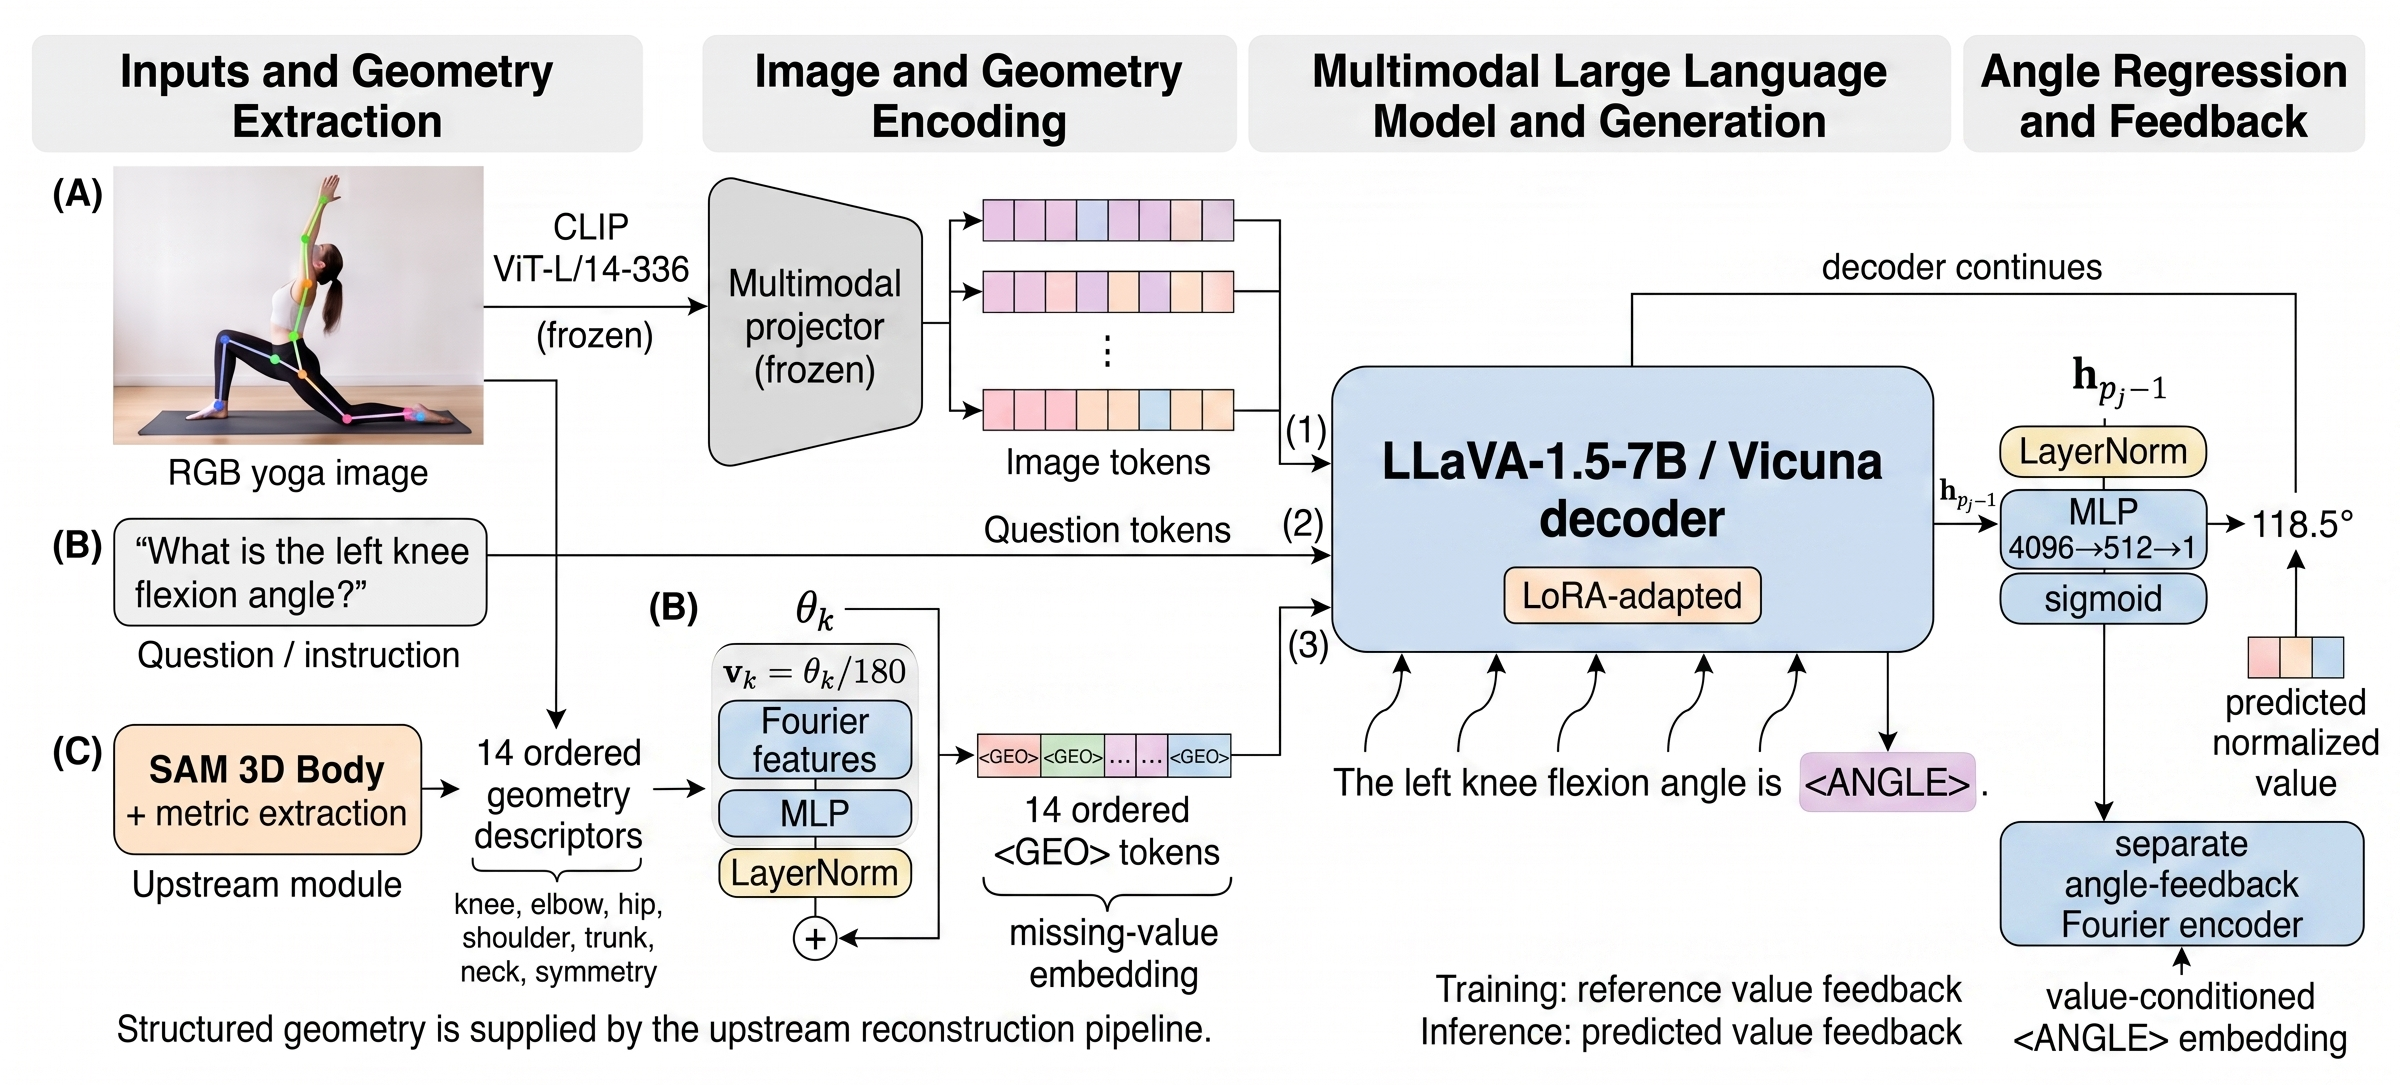
\includegraphics[width=0.98\textwidth]{method.png}
    \caption{Overview of YogaLLaVA V3. An input image is encoded by the frozen
    LLaVA visual pathway, while an ordered set of degree-valued body descriptors
    is mapped to metric-aware \texttt{<GEO>} tokens. The causal language decoder
    attends jointly to visual, geometric, and textual context. When the decoder
    emits an \texttt{<ANGLE>} token, a regression head predicts the associated
    continuous value, which is embedded back into the sequence to condition
    subsequent generation.}
    \label{fig:yogallava_architecture}
\end{figure*}

\subsection{Structured Geometry Input}
\label{sec:structured_geometry_input}

YogaLLaVA V3 uses a fixed vocabulary of $K=14$ degree-valued descriptors:
left and right knee flexion, left and right elbow flexion, left and right hip
opening, left and right shoulder elevation, trunk tilt, lateral trunk bend,
trunk twist, neck alignment, knee symmetry, and elbow symmetry. These
descriptors form the angular subset of the broader geometric taxonomy introduced
in Sec.~\ref{sec:dataset}. Scale-dependent quantities, such as stance width and
body-center offset, are not supplied to the model. Hip symmetry is likewise not
represented by a dedicated input descriptor, although three hip-symmetry
targets occur in the held-out test set.

We represent the ordered geometry input as
\begin{equation}
    \mathcal{G}
    =
    \left\{(\theta_k,m_k)\right\}_{k=1}^{K},
    \qquad m_k\in\{0,1\},
    \label{eq:geometry_input}
\end{equation}
where $\theta_k$ is the $k$-th descriptor in degrees and $m_k$ indicates
whether that measurement is available. Explicitly modeling validity is
necessary because a missing measurement is semantically distinct from a valid
angle close to zero.

\subsection{Multimodal Geometry Representation}
\label{sec:geometry_representation}

\noindent\textbf{Visual and language pathways.}
The image is processed by the pretrained CLIP ViT-L/14-336 vision encoder in
LLaVA. Its patch-level features are projected into the language-model hidden
space through the frozen multimodal projector. The instruction and question are
tokenized using the LLaVA tokenizer and combined with the projected visual
features through the standard LLaVA multimodal interface.

To inject structured geometry, we append exactly $K$ special
\texttt{<GEO>} placeholders in a fixed canonical order. Before decoding, the
ordinary embeddings of these placeholders are replaced by geometry
representations with the same dimensionality as the language-model hidden
states. Consequently, visual features, text tokens, and structured measurements
are processed within a shared autoregressive sequence.

\noindent\textbf{Fourier encoding of continuous measurements.}
For every available descriptor, we normalize its value to $[0,1]$:
\begin{equation}
    v_k=\frac{\theta_k}{180}.
    \label{eq:angle_normalization}
\end{equation}
Rather than applying a single linear projection to $v_k$, we encode it using
$B=16$ fixed, logarithmically spaced Fourier frequency bands:
\begin{equation}
\begin{split}
    \boldsymbol{\phi}(v_k)=\big[
        &\sin(\omega_1v_k),\ldots,\sin(\omega_Bv_k),\\
        &\cos(\omega_1v_k),\ldots,\cos(\omega_Bv_k),v_k
    \big].
\end{split}
\label{eq:fourier_features}
\end{equation}
This mapping produces a $(2B+1)=33$ dimensional representation. A two-layer
MLP with hidden width 256 projects it to the $d=4096$ dimensional
language-model space:
\begin{equation}
    \mathbf{z}_k
    =f_{\mathrm{geo}}\!\left(\boldsymbol{\phi}(v_k)\right),
    \qquad \mathbf{z}_k\in\mathbb{R}^{d}.
    \label{eq:scalar_projection}
\end{equation}

\noindent\textbf{Metric identity and missing values.}
The same scalar may carry different meanings for different anatomical
measurements. We therefore associate each descriptor with a learned
metric-identity embedding $\mathbf{e}^{\mathrm{id}}_k\in\mathbb{R}^{d}$.
The final token for descriptor $k$ is
\begin{equation}
    \mathbf{g}_k=
    \begin{cases}
    \operatorname{LN}\!\left(
        \mathbf{e}^{\mathrm{id}}_k+\mathbf{z}_k
    \right), & m_k=1,\\[5pt]
    \operatorname{LN}\!\left(
        \mathbf{e}^{\mathrm{id}}_k+\mathbf{e}^{\mathrm{miss}}
    \right), & m_k=0,
    \end{cases}
    \label{eq:geometry_token}
\end{equation}
where $\mathbf{e}^{\mathrm{miss}}\in\mathbb{R}^{d}$ is a learned missing-value
embedding and $\operatorname{LN}$ denotes layer normalization. The ordered
geometry sequence is therefore
\begin{equation}
    \mathbf{G}=[\mathbf{g}_1,\ldots,\mathbf{g}_K]
    \in\mathbb{R}^{K\times d}.
    \label{eq:geometry_sequence}
\end{equation}
These vectors replace the corresponding \texttt{<GEO>} embeddings, enabling
the decoder to attend jointly to the image, question, and metric-specific
continuous geometry.

\subsection{Angle-Aware Language Generation}
\label{sec:angle_generation}

Standard language models express numbers through discrete subword tokens, which
does not provide an explicit continuous prediction objective. YogaLLaVA V3
instead introduces a special \texttt{<ANGLE>} token that separates numeric-slot
placement from scalar-value estimation. During training, every degree value in
a geometry-grounded answer is replaced by \texttt{<ANGLE>}, and its normalized
value is retained as a continuous target aligned with that token position. For
example,
\begin{quote}
\small
\textit{The left knee flexion angle is $140.2^\circ$.}
\end{quote}
is represented internally as
\begin{quote}
\small
\texttt{The left knee flexion angle is <ANGLE>.}
\end{quote}
The language decoder thus learns \emph{where} an angular value is required,
whereas the regression branch learns \emph{which} value should occupy that
position.

Let $p_j$ denote the position of the $j$-th \texttt{<ANGLE>} token. Under causal
decoding, the hidden state $\mathbf{h}_{p_j-1}$ produces the token at position
$p_j$. We predict its normalized value as
\begin{equation}
    \widehat{v}_j
    =\sigma\!\left(
        f_{\mathrm{reg}}(\mathbf{h}_{p_j-1})
    \right),
    \label{eq:angle_regression}
\end{equation}
where $f_{\mathrm{reg}}$ comprises layer normalization, a
$4096\!\rightarrow\!512$ linear layer, GELU, and a
$512\!\rightarrow\!1$ linear layer. The sigmoid restricts predictions to
$[0,1]$, after which the angle is recovered in degrees:
\begin{equation}
    \widehat{\theta}_j=180\widehat{v}_j.
    \label{eq:angle_denormalization}
\end{equation}
Using $\mathbf{h}_{p_j-1}$ ensures that the current value is estimated from the
preceding causal context, rather than from a value-conditioned embedding placed
at the current \texttt{<ANGLE>} position.

\noindent\textbf{Continuous-value feedback.}
After an angle slot is produced, its scalar value is re-embedded into the
sequence so that subsequent language and later angle slots may condition on it.
An independent scalar encoder defines
\begin{equation}
    \mathbf{a}(u_j)
    =\mathbf{e}^{\mathrm{angle}}
    +f_{\mathrm{slot}}\!\left(\boldsymbol{\phi}(u_j)\right),
    \label{eq:angle_feedback}
\end{equation}
where $\mathbf{e}^{\mathrm{angle}}$ is a learned base embedding and
$f_{\mathrm{slot}}$ is distinct from the geometry-input encoder
$f_{\mathrm{geo}}$. During teacher-forced training, $u_j$ is the reference
normalized angle; during autoregressive inference, $u_j=\widehat{v}_j$.
Accordingly, subsequent tokens condition on the reference value during training
and on the model's own prediction at inference time.

\subsection{Joint Language and Geometry Learning}
\label{sec:training_objective}

We jointly optimize natural-language generation and continuous angle
prediction. Language supervision is restricted to the assistant response; image
and geometry placeholders, the instruction, the question, and padding positions
are excluded. Let $\mathcal{T}$ denote the supervised assistant-token positions.
The causal language-modeling objective is
\begin{equation}
    \mathcal{L}_{\mathrm{LM}}
    =-\frac{1}{|\mathcal{T}|}
    \sum_{t\in\mathcal{T}}
    \log p_{\Theta}\!\left(
        y_t\mid y_{<t},I,q,\mathcal{G}
    \right).
    \label{eq:language_loss}
\end{equation}

For a minibatch containing $N$ supervised angle slots, the regression branch is
optimized in normalized angle space using
\begin{equation}
    \mathcal{L}_{\mathrm{ang}}
    =\frac{1}{N}\sum_{j=1}^{N}
    \operatorname{SmoothL1}_{\beta}
    \!\left(\widehat{v}_j-v_j\right).
    \label{eq:regression_loss}
\end{equation}
The complete training objective is
\begin{equation}
    \mathcal{L}
    =\mathcal{L}_{\mathrm{LM}}
    +\lambda_{\mathrm{ang}}\mathcal{L}_{\mathrm{ang}},
    \label{eq:total_loss}
\end{equation}
with $\lambda_{\mathrm{ang}}=0.75$ and $\beta=0.05$, corresponding to a
$9^\circ$ SmoothL1 transition in degree space. The language term is implemented
as causal cross-entropy with label smoothing. Domain-knowledge records contain
no \texttt{<ANGLE>} positions and therefore contribute only
$\mathcal{L}_{\mathrm{LM}}$.

To reduce complete dependence on structured measurements, we apply full
geometry dropout to 15\% of geometry-grounded training records. For a selected
record, every measurement is marked unavailable and represented by the learned
missing-value embedding.

The CLIP vision encoder and multimodal projector remain frozen. We adapt the
Vicuna language decoder using LoRA with rank 32, scaling parameter 64, and
dropout 0.10. LoRA is applied to the $q$, $k$, $v$, and $o$ attention
projections and to the gate, up, and down feed-forward projections. The geometry
encoder, angle-feedback encoder, learned angle embedding, regression head, and
LoRA parameters are optimized jointly. After adding \texttt{<GEO>} and
\texttt{<ANGLE>} to the vocabulary, the input-embedding matrix and
language-model output projection are also trainable.

\subsection{Autoregressive Inference}
\label{sec:inference}

At inference time, the upstream reconstruction pipeline provides the ordered
geometry descriptors, while the LLaVA visual pathway encodes the input image.
The image, geometry tokens, instruction, and question are supplied without a
reference answer.

Decoding proceeds autoregressively. Ordinary tokens follow the standard LLaVA
generation process. When \texttt{<ANGLE>} is selected, the hidden state that
produced it is passed to the regression head to obtain $\widehat{v}_j$. The
prediction is converted to degrees for the final response and encoded through
Eq.~\eqref{eq:angle_feedback} as the embedding of the emitted
\texttt{<ANGLE>} token before decoding resumes. After generation, the
placeholders are replaced in order by their predicted degree values. Token
probabilities and scalar predictions are therefore not averaged or combined at
the output level; they interact through the slot-emission and continuous-value
feedback mechanism.

\section{Experiments}
\label{sec:experimental_setup}

\subsection{Data Splits}
\label{sec:dataset_splits}

We evaluate YogaLLaVA V3 on the combined domain-knowledge and
geometry-grounded QA corpus introduced in Sec.~\ref{sec:dataset}. The fixed
splits contain 10,090 records and 10,177 supervised angle slots
(Table~\ref{tab:dataset_splits}). The geometry-grounded subset is constructed
from 3,000 images, with two QA records per image, and comprises 3,000
direct-angle, 905 comparison, 900 regional-summary, 600 misconception, and 595
instructor-observation examples. Test images are excluded from training, while
pose categories are shared across splits. The resulting protocol evaluates
generalization to unseen images of known asanas rather than to unseen pose
categories.

\begin{table}[t]
    \centering
    \caption{Composition of the instruction-tuning corpus.}
    \label{tab:dataset_splits}
    \resizebox{\columnwidth}{!}{
    \begin{tabular}{lrrrr}
        \toprule
        \textbf{Split} &
        \textbf{Geometry QA} &
        \textbf{Domain QA} &
        \textbf{Total} &
        \textbf{Angle Slots} \\
        \midrule
        Train      & 5,396 & 3,690 & 9,086 & 9,163 \\
        Validation &   294 &   200 &   494 &   493 \\
        Test       &   310 &   200 &   510 &   521 \\
        \midrule
        Total      & 6,000 & 4,090 & 10,090 & 10,177 \\
        \bottomrule
    \end{tabular}}
\end{table}

\subsection{Implementation Details}
\label{sec:implementation_details}

YogaLLaVA V3 is initialized from LLaVA-1.5-7B. Its CLIP ViT-L/14-336
image encoder operates at $336\!\times\!336$ resolution, and the multimodal
projector maps the visual features to the 4,096-dimensional language space.
The maximum sequence length is 1,280 tokens. Both the vision encoder and
multimodal projector remain frozen; the language decoder is adapted using the
LoRA configuration described in Sec.~\ref{sec:training_objective}, together
with the proposed geometry and angle modules.

We train for 12 epochs using AdamW with weight decay 0.01 and gradient clipping
at 1.0. A per-device batch size of four and eight-step gradient accumulation
produce an effective batch size of 32. We use a cosine learning-rate schedule
with linear warm-up over the first 3\% of optimizer updates. The learning rates
are $1.5\!\times\!10^{-4}$ for LoRA parameters,
$2\!\times\!10^{-5}$ for the trainable input and output embeddings, and
$1\!\times\!10^{-4}$ for the geometry encoder, angle-feedback encoder, angle
embedding, and regression head. The pretrained backbone is loaded in bfloat16,
whereas the custom numeric modules are maintained in float32. Training is
performed on one NVIDIA RTX A6000 GPU with fixed Python, NumPy, PyTorch, and
CUDA seeds.

We evaluate the model after every epoch and select the checkpoint with the
lowest teacher-forced validation angle RMSE. The selected checkpoint obtains a
validation RMSE of $19.83^\circ$, MAE of $12.63^\circ$, and $R^2$ of 0.874.
We report only the selected checkpoint because intermediate epoch-wise values
are optimization diagnostics rather than comparative experimental results.

\subsection{Evaluation Protocol}
\label{sec:evaluation_protocol}

\noindent\textbf{Teacher-forced angle regression.}
Our primary numeric evaluation supplies the reference answer structure,
including the number, positions, and ordering of \texttt{<ANGLE>} tokens, and
evaluates the continuous prediction at each known slot. Given $N$ reference
angles $\theta_i$ and predictions $\widehat{\theta}_i$, we report MAE, RMSE,
$R^2$, Pearson correlation, and the fractions of predictions within
$5^\circ$, $10^\circ$, and $15^\circ$ of the references:
\begin{equation}
\operatorname{MAE}=\frac{1}{N}\sum_{i=1}^{N}
\left|\widehat{\theta}_i-\theta_i\right|,
\qquad
\operatorname{RMSE}=\sqrt{\frac{1}{N}\sum_{i=1}^{N}
(\widehat{\theta}_i-\theta_i)^2}.
\label{eq:evaluation_errors}
\end{equation}
Teacher forcing isolates continuous prediction given the correct linguistic
slot structure; it does not evaluate whether the model can autonomously emit,
order, and contextualize the required slots.

\noindent\textbf{Autoregressive generation.}
We therefore additionally evaluate free-running generation on all 310
geometry-grounded test records. YogaLLaVA V3 receives the image, question, and
structured geometry. LLaVA-1.5-7B and Qwen2.5-VL-7B-Instruct~\cite{bai2025qwen25vl} are evaluated
zero-shot using only the image and question; the questions specify the target
metrics and their expected order but do not reveal numeric values. We report
(i) slot-count accuracy over the complete test set and (ii) numeric error on
the common-success subset for which all models generate the correct number of
values. This distinction avoids directly comparing numeric errors computed on
different model-specific subsets.

All numeric references are pseudo-measurements derived from SAM 3D Body rather
than motion capture or manually verified biomechanical annotations. Moreover,
518 of the 521 teacher-forced test targets are present in the structured
geometry input. The primary evaluation therefore measures question-conditioned
descriptor selection, routing, reproduction, and linguistic expression, not
independent physical angle recovery from RGB images.

\section{Results}
\label{sec:results}

\subsection{Overall Angle-Slot Regression}
\label{sec:overall_results}

Table~\ref{tab:overall_results} summarizes teacher-forced regression over 521
angle slots from 310 held-out geometry-grounded records. YogaLLaVA V3 obtains
an MAE of $13.98^\circ$ and an RMSE of $21.82^\circ$, with a Pearson
correlation of 0.913. In addition, 57.01\% and 70.63\% of predictions fall
within $10^\circ$ and $15^\circ$, respectively, of the reconstruction-derived
references. These results indicate that the model can identify and express the
requested measurement from the supplied geometry under a known answer
structure.

\begin{table}[t]
    \centering
    \caption{Teacher-forced angle-slot regression on the held-out test set.
    Errors are measured against SAM 3D Body-derived pseudo-measurements.}
    \label{tab:overall_results}
    \begin{tabular}{lr}
        \toprule
        \textbf{Metric} & \textbf{YogaLLaVA V3} \\
        \midrule
        Angle slots & 521 \\
        RMSE $\downarrow$ & $21.82^\circ$ \\
        MAE $\downarrow$ & $13.98^\circ$ \\
        $R^2$ $\uparrow$ & 0.832 \\
        Pearson $r$ $\uparrow$ & 0.913 \\
        Within $5^\circ$ $\uparrow$ & 34.36\% \\
        Within $10^\circ$ $\uparrow$ & 57.01\% \\
        Within $15^\circ$ $\uparrow$ & 70.63\% \\
        \bottomrule
    \end{tabular}
\end{table}

\subsection{Analysis by Question Type}
\label{sec:path_results}

Table~\ref{tab:path_results} reports performance across the five geometry-QA
families. Misconception questions achieve the lowest MAE
($11.28^\circ$) and highest within-$10^\circ$ accuracy (68.75\%), although
this subset contains only 32 slots. Regional-summary and comparison questions
also perform favorably despite requiring multiple values or cross-body-part
relations. Instructor-observation questions are the most challenging, with an
MAE of $21.08^\circ$ and within-$10^\circ$ accuracy of 25.81\%. Their less
explicit teacher-style formulations may make descriptor selection more
ambiguous, although the present experiment does not isolate this factor.

\begin{table}[t]
    \centering
    \caption{Teacher-forced regression by geometry-QA type.}
    \label{tab:path_results}
    \resizebox{\columnwidth}{!}{
    \begin{tabular}{lrrrrr}
        \toprule
        \textbf{Question Type} & \textbf{Slots} &
        \textbf{RMSE $\downarrow$} & \textbf{MAE $\downarrow$} &
        \textbf{$R^2$ $\uparrow$} & \textbf{$\leq10^\circ$ $\uparrow$} \\
        \midrule
        Comparison & 106 & $21.53^\circ$ & $12.95^\circ$ & 0.791 & 62.26\% \\
        Direct angle & 155 & $22.65^\circ$ & $15.22^\circ$ & 0.821 & 51.61\% \\
        Instructor observation & 31 & $28.69^\circ$ & $21.08^\circ$ & 0.054 & 25.81\% \\
        Misconception & 32 & $17.10^\circ$ & $11.28^\circ$ & 0.877 & 68.75\% \\
        Region summary & 197 & $20.72^\circ$ & $12.88^\circ$ & 0.847 & 61.42\% \\
        \bottomrule
    \end{tabular}}
\end{table}

\subsection{Analysis by Geometric Descriptor}
\label{sec:metric_results}

Among descriptors with substantial test support, trunk twist yields the lowest
MAE ($6.84^\circ$), followed by lateral trunk bend, trunk tilt, and right
shoulder elevation (Table~\ref{tab:metric_results}). Left shoulder elevation is
the most difficult descriptor, followed by elbow flexion and right hip opening.
These differences may arise from descriptor-specific distributions,
reconstruction uncertainty, occlusion, or left--right ambiguity; identifying
their individual effects requires further controlled analysis.

The symmetry categories contain only three or four slots and should not be used
to draw broad conclusions. Hip symmetry is additionally distinct because no
dedicated hip-symmetry token is included in the 14-descriptor input vocabulary;
its three test targets therefore cannot be retrieved from a corresponding
independent input token.

\begin{table}[t]
    \centering
    \caption{Teacher-forced regression by target descriptor.}
    \label{tab:metric_results}
    \resizebox{\columnwidth}{!}{
    \begin{tabular}{lrrr}
        \toprule
        \textbf{Descriptor} & \textbf{Slots} &
        \textbf{RMSE $\downarrow$} & \textbf{MAE $\downarrow$} \\
        \midrule
        Knee symmetry & 4 & $3.23^\circ$ & $2.68^\circ$ \\
        Elbow symmetry & 4 & $6.90^\circ$ & $5.53^\circ$ \\
        Hip symmetry & 3 & $10.18^\circ$ & $7.82^\circ$ \\
        Trunk twist & 33 & $11.02^\circ$ & $6.84^\circ$ \\
        Lateral trunk bend & 38 & $14.92^\circ$ & $9.24^\circ$ \\
        Right shoulder elevation & 34 & $14.82^\circ$ & $9.89^\circ$ \\
        Trunk tilt & 34 & $15.48^\circ$ & $9.50^\circ$ \\
        Neck alignment & 37 & $17.34^\circ$ & $12.75^\circ$ \\
        Left hip opening & 48 & $18.40^\circ$ & $13.28^\circ$ \\
        Right knee flexion & 51 & $22.55^\circ$ & $12.09^\circ$ \\
        Left knee flexion & 47 & $23.66^\circ$ & $15.56^\circ$ \\
        Right elbow flexion & 50 & $24.80^\circ$ & $18.39^\circ$ \\
        Right hip opening & 48 & $25.41^\circ$ & $17.36^\circ$ \\
        Left elbow flexion & 47 & $27.77^\circ$ & $18.46^\circ$ \\
        Left shoulder elevation & 43 & $31.22^\circ$ & $21.23^\circ$ \\
        \bottomrule
    \end{tabular}}
\end{table}

\subsection{Autoregressive Generation}
\label{sec:generation_comparison}

Table~\ref{tab:generation_results} evaluates complete free-running generation.
YogaLLaVA V3 emits the correct number of numeric values for 267 of 310 records
(86.1\%), compared with 66.1\% for LLaVA-1.5-7B and 68.1\% for
Qwen2.5-VL-7B. Thus, the proposed model is more reliable at determining when
and how many continuous outputs are required.

For numeric comparison, we use the 160-record common-success subset on which
all three models produce the correct slot count. YogaLLaVA V3 achieves a
slot-level MAE of $17.65^\circ$, substantially below LLaVA
($42.80^\circ$) and Qwen ($46.91^\circ$). Its record-level macro MAE is
$16.98^\circ$ with a 95\% bootstrap confidence interval of
$[14.15,20.17]^\circ$. The corresponding intervals are
$[37.33,46.41]^\circ$ for LLaVA and $[41.59,53.87]^\circ$ for Qwen.
Paired bootstrap differences relative to YogaLLaVA are
$24.85^\circ$ ($[19.45,30.35]^\circ$) for LLaVA and
$30.64^\circ$ ($[23.70,37.83]^\circ$) for Qwen.

\begin{table}[t]
    \centering
    \caption{Autoregressive generation on 310 test records. Slot accuracy is
    measured on the full test set; numeric errors use the 160-record
    common-success subset.}
    \label{tab:generation_results}
    \resizebox{\columnwidth}{!}{
    \begin{tabular}{lrrr}
        \toprule
        \textbf{Model} & \textbf{Slot Match $\uparrow$} &
        \textbf{MAE $\downarrow$} & \textbf{RMSE $\downarrow$} \\
        \midrule
        YogaLLaVA V3 & 267/310 (86.1\%) & $17.65^\circ$ & $27.23^\circ$ \\
        LLaVA-1.5-7B & 205/310 (66.1\%) & $42.80^\circ$ & $52.59^\circ$ \\
        Qwen2.5-VL-7B & 211/310 (68.1\%) & $46.91^\circ$ & $61.12^\circ$ \\
        \bottomrule
    \end{tabular}}
\end{table}

This comparison evaluates complete systems rather than isolating a single
architectural factor. YogaLLaVA V3 receives structured geometry and
task-specific instruction tuning, whereas the baselines are image-only and
zero-shot. The observed advantage therefore reflects the combined effect of
geometry conditioning, domain adaptation, and continuous angle regression; it
should not be interpreted as a modality-matched ablation.

\subsection{Discussion and Limitations}
\label{sec:result_interpretation}

The teacher-forced and autoregressive evaluations characterize complementary
capabilities. The former measures continuous prediction at known answer slots,
whereas the latter additionally requires the model to decide whether a numeric
slot is needed, emit and order the correct number of slots, preserve consistency
between numbers and language, and terminate appropriately. Reporting them
separately avoids conflating regression accuracy with complete generation
quality.

The current evidence supports geometry-conditioned measurement selection and
expression, but not independent image-only recovery of physical joint angles.
The references inherit uncertainty from monocular reconstruction, including
viewpoint, occlusion, foreshortening, clothing, inversion, depth, and
left--right ambiguities. They should therefore not be interpreted as clinical,
diagnostic, rehabilitation, motion-capture, or manually verified biomechanical
ground truth. Finally, the experiments do not isolate modality contributions
through ablation and do not test generalization to unseen yoga-pose categories;
both remain important directions for future evaluation.

\section{Conclusion}
\label{sec:conclusion}

We introduced YogaAlign, a geometry-grounded extension of Yoga-82, and
YogaLLaVA V3, a vision--language model that integrates structured body
measurements with continuous angle-aware generation. YogaAlign combines
pose-level domain knowledge with image-specific QA derived from explicit
reconstruction-based evidence paths. YogaLLaVA V3 represents these measurements
as metric-aware geometry tokens and predicts continuous values at dedicated
angle slots. The experiments demonstrate reliable question-conditioned
selection and expression of supplied geometry under both teacher-forced and
autoregressive evaluation. They also define the present scope clearly: the
system reasons over monocular reconstruction-derived measurements and is not a
substitute for independently validated biomechanical assessment. Future work
should evaluate modality-matched ablations, human-verified geometric references,
pose-held-out generalization, and the consistency of generated corrections with
expert instruction.

\bibliographystyle{IEEEtran}
\bibliography{references}

\end{document}
